\documentclass[11pt,a4paper]{article}
\usepackage{pgfplots}
\usetikzlibrary{positioning}
\usetikzlibrary{fit}
\usetikzlibrary{backgrounds}
\usetikzlibrary{calc}
\usetikzlibrary{shapes}
\usetikzlibrary{mindmap}
\usetikzlibrary{decorations.text}
\usepackage[authoryear, round]{natbib}
\usepackage[T1]{fontenc}
\usepackage{lmodern}
\usepackage{amssymb,amsmath}
\usepackage{ifxetex,ifluatex}
\usepackage{fixltx2e} % provides \textsubscript
% use upquote if available, for straight quotes in verbatim environments
\IfFileExists{upquote.sty}{\usepackage{upquote}}{}
\ifnum 0\ifxetex 1\fi\ifluatex 1\fi=0 % if pdftex
  \usepackage[utf8]{inputenc}
\else % if luatex or xelatex
  \ifxetex
    \usepackage{mathspec}
    \usepackage{xltxtra,xunicode}
  \else
    \usepackage{fontspec}
  \fi
  \defaultfontfeatures{Mapping=tex-text,Scale=MatchLowercase}
  \newcommand{\euro}{€}
\fi
% use microtype if available
\IfFileExists{microtype.sty}{\usepackage{microtype}}{}
\usepackage{color}
\usepackage{fancyvrb}
\newcommand{\VerbBar}{|}
\newcommand{\VERB}{\Verb[commandchars=\\\{\}]}
\DefineVerbatimEnvironment{Highlighting}{Verbatim}{commandchars=\\\{\}}
% Add ',fontsize=\small' for more characters per line
\usepackage{framed}
\definecolor{shadecolor}{RGB}{248,248,248}
\newenvironment{Shaded}{\begin{snugshade}}{\end{snugshade}}
\newcommand{\KeywordTok}[1]{\textcolor[rgb]{0.13,0.29,0.53}{\textbf{{#1}}}}
\newcommand{\DataTypeTok}[1]{\textcolor[rgb]{0.13,0.29,0.53}{{#1}}}
\newcommand{\DecValTok}[1]{\textcolor[rgb]{0.00,0.00,0.81}{{#1}}}
\newcommand{\BaseNTok}[1]{\textcolor[rgb]{0.00,0.00,0.81}{{#1}}}
\newcommand{\FloatTok}[1]{\textcolor[rgb]{0.00,0.00,0.81}{{#1}}}
\newcommand{\CharTok}[1]{\textcolor[rgb]{0.31,0.60,0.02}{{#1}}}
\newcommand{\StringTok}[1]{\textcolor[rgb]{0.31,0.60,0.02}{{#1}}}
\newcommand{\CommentTok}[1]{\textcolor[rgb]{0.56,0.35,0.01}{\textit{{#1}}}}
\newcommand{\OtherTok}[1]{\textcolor[rgb]{0.56,0.35,0.01}{{#1}}}
\newcommand{\AlertTok}[1]{\textcolor[rgb]{0.94,0.16,0.16}{{#1}}}
\newcommand{\FunctionTok}[1]{\textcolor[rgb]{0.00,0.00,0.00}{{#1}}}
\newcommand{\RegionMarkerTok}[1]{{#1}}
\newcommand{\ErrorTok}[1]{\textbf{{#1}}}
\newcommand{\NormalTok}[1]{{#1}}
\usepackage{graphicx}
% Redefine \includegraphics so that, unless explicit options are
% given, the image width will not exceed the width of the page.
% Images get their normal width if they fit onto the page, but
% are scaled down if they would overflow the margins.
\makeatletter
\def\ScaleIfNeeded{%
  \ifdim\Gin@nat@width>\linewidth
    \linewidth
  \else
    \Gin@nat@width
  \fi
}
\makeatother
\let\Oldincludegraphics\includegraphics
{%
 \catcode`\@=11\relax%
 \gdef\includegraphics{\@ifnextchar[{\Oldincludegraphics}{\Oldincludegraphics[width=\ScaleIfNeeded]}}%
}%
\ifxetex
  \usepackage[setpagesize=false, % page size defined by xetex
              unicode=false, % unicode breaks when used with xetex
              xetex]{hyperref}
\else
  \usepackage[unicode=true]{hyperref}
\fi
\hypersetup{breaklinks=true,
            bookmarks=true,
            pdfauthor={},
            pdftitle={Data management procedures for reproducible research pipelines},
            colorlinks=true,
            citecolor=black,
            urlcolor=black,
            linkcolor=black,
            pdfborder={0 0 0}}
\urlstyle{same}  % don't use monospace font for urls
\setlength{\parindent}{0pt}
\setlength{\parskip}{6pt plus 2pt minus 1pt}
\setlength{\emergencystretch}{3em}  % prevent overfull lines
\setcounter{secnumdepth}{5}

%%%%%%%%%%%%%%%%%%%%%%%%%%%%%%%%%%%%%%%%%%%%%%%%%%%%%%%%
%Changes borrowed from @cboettig, added by @jhollist 
% A modified page layout 
\textwidth 6.75in
\oddsidemargin -0.15in
\evensidemargin -0.15in
\textheight 9in
\topmargin -0.5in
\usepackage{lineno} % add 
%%%%%%%%%%%%%%%%%%%%%%%%%%%%%%%%%%%%%%%%%%%%%%%%%%%%%%%%

%%%%%%%%%%%%%%%%%%%%%%%%%%%%%%%%%%%%%%%%%%%%%%%%%%%%%%%%
%%Packages and layout changes by @jhollist 09/15/2014
\usepackage{ragged2e}
\usepackage[font=normalsize]{caption}
  \usepackage[singlespacing]{setspace}
\usepackage{parskip}
\usepackage{fancyhdr}
\pagestyle{fancy}
\fancyhf{}
\renewcommand{\headrulewidth}{0pt}
%\rfoot{\today}
\cfoot{\thepage}
%%Changed default abstract width and added lines
\renewenvironment{abstract}{
  \hfill\begin{minipage}{1\textwidth}
  \rule{\textwidth}{1pt}\vspace{5pt}
  \normalsize
  \begin{justify}
  \bfseries\abstractname\vspace{5pt}
  \end{justify}}
  {\par\noindent\rule{\textwidth}{1pt}\end{minipage}
}
%%%%%%%%%%%%%%%%%%%%%%%%%%%%%%%%%%%%%%%%%%%%%%%%%%%%%%%%

\title{Data management procedures for \\ reproducible research pipelines}
\author{
Ivan C. Hanigan
}
\date{}
\usepackage{graphicx}
\usepackage{url}
\usepackage{hyperref}
\usepackage{tikz}
\usetikzlibrary{calc}


\usepackage{hyperref}

\usetikzlibrary{calc}

\usepackage{tikz}
%------------------%
\makeatletter
\newcount\dirtree@lvl
\newcount\dirtree@plvl
\newcount\dirtree@clvl
\def\dirtree@growth{%
  \ifnum\tikznumberofcurrentchild=1\relax
  \global\advance\dirtree@plvl by 1
  \expandafter\xdef\csname dirtree@p@\the\dirtree@plvl\endcsname{\the\dirtree@lvl}
  \fi
  \global\advance\dirtree@lvl by 1\relax
  \dirtree@clvl=\dirtree@lvl
  \advance\dirtree@clvl by -\csname dirtree@p@\the\dirtree@plvl\endcsname
  \pgf@xa=0.5cm\relax % change the length to your needs
  \pgf@ya=-0.75cm\relax % change the length to your needs
  \pgf@ya=\dirtree@clvl\pgf@ya
  \pgftransformshift{\pgfqpoint{\the\pgf@xa}{\the\pgf@ya}}%
  \ifnum\tikznumberofcurrentchild=\tikznumberofchildren
  \global\advance\dirtree@plvl by -1
  \fi
}
\tikzset{ %definition of a new style "dirtree"
  dirtree/.style={
    growth function=\dirtree@growth,
    every node/.style={anchor=north},
    every child node/.style={anchor=west},
    edge from parent path={(\tikzparentnode\tikzparentanchor) |- (\tikzchildnode\tikzchildanchor)}
  }
}
\makeatother

\begin{document}
\begin{singlespace}
\begin{center}
\huge Data management procedures \\ for reproducible research pipelines
\end{center}
%%Adds Author, correspond email asterisk, and affilnum from YAML
\begin{center}
\large Ivan C. Hanigan
\end{center}
%%Adds affiliations from YAML
\begin{justify}
\footnotesize \emph{ 
}
%%Adds corresponding author email(s) from YAML
\newcounter{num}
\setcounter{num}{1}
\\[0.1cm]
\footnotesize \emph{ 
}
\end{justify}
%%Adds date from YAML
\normalsize

\begin{abstract}
This unpublished working paper was written to accompany the material included in the PhD thesis `Using Reproducible Research Pipelines to Help Disentangle Health Effects of Environmental Changes from Social Factors' by Ivan Hanigan (2016). It sets out the key data management and analysis principles that were found to be most effective for the reproducibile synthesis and integration of
heterogeneous datasets for analysis and reporting. The draft was last updated \today. The version submitted with the thesis is available on the phd\_appendix branch of the Github repository: \url{https://github.com/swish-climate-impact-assessment/swish_data_management_procedures}.
\end{abstract}
\end{singlespace}

{
\hypersetup{linkcolor=black}
\setcounter{tocdepth}{2}
\tableofcontents
}

\clearpage
%\doublespace

\section{Introduction}\label{introduction}

There is a need for developing an evidence-based set of best practice
guidelines for data management procedures that support reproducibility in all fields of computational data analysis \citep{Long2008,Noble2009,Peng}. 
Reproducibility is the ability to recompute the results of a data
analysis with the original data (as distinct from replication which involves analysing independently collected data \citep{Peng2011}). 
The examples drawn
together in this report come from experiences and use-cases found from implementing reproducible
research pipelines in an
eco-social epidemiologic research context. This emerging paradigm 
mixes environmental and social epidemiology and is inherently concerned with complex systems. To do this work 
integration of heterogenous data sources, and synthesising new datasets, is required.  Then analyses that aim to  recognise subtle and complicated patterns in
the environmental and social determinants of health must be rigorously and transparently conducted
\citep{McMichael2013}. This document outlines a suite of data management
procedures that have been found to effectively assist the development of
reproducible research pipelines in this context.

\subsection{The 'reproducibility crisis'}

It is possible to have analyses that
are reproducible with varying degrees of difficulty. A data analysis
might be reproducible but require thousands of hours of work. A primary
challenge for reproducible data analysis is to make analyses that are
\emph{easy} to reproduce.

In essence this requires attention to be turned to the issue of how the
data and analytical steps amassed -- toward a reality where this is
archived and there is a good understanding all round as to how the study
were set up and conducted. Different assumptions or different treatment
of the data could conceivably lead to different inferences and
conclusions being drawn, such as in the example shown by \citet{Silberzahn2015} in which 29 research teams were given the same dataset
but reached a wide variety of conclusions using different methods on the
same dataset to answer the same question.

This is partly because of an underlying complexity in the information
drawn from complex systems involving multi-causality, and partly because
of different assumptions and different backgrounds and viewpoints. A
finding that a variable does or does not cause a disease, might be drawn
honestly from the same set of data.


\subsection{A common (flawed) approach for generating statistical reports}

A common approach with inherent flaws that make it error-prone was identified by \citet{Scott}, and the examples are paraphrased here.  
First, the data entry, cleaning, preparation and possibly statistical analyses are conducted by 'point-and-click' procedures using software such as Microsoft (MS) Excel.
This introduces well-known issues with handling of missing data, poor algorithms and unreliable results \citep{McCullough2008}.
In cases where data are imported to a program such as STATA or SPSS, further point-and-click data preparation and statistical analyses often occur.
Spreadsheet software such as MS Excel is regularly used to record or format the desired results, and generate figures.
Finally, the results (text, tables and figures) from the data analysis system are inserted into a word processor (eg, MS Word) using 'copy-and-paste' procedures (or typed by hand). 
\clearpage
Problems with this common, flawed approach according to \citet{Scott} are:
\begin{itemize}
\item You sit down to finish writing your manuscript. You realize that you need to clarify one result by running an additional analysis. You first re-run the primary analysis. Major problem: the primary results don’t match what you have in your paper.
\item When you go to your project folder to run the additional analysis, you find multiple data files, multiple analysis files,
and multiple results files. You can’t remember which ones are pertinent.
\item You\'ve just spent the week running your analysis and creating a results report (including tables and figures) to present to your collaborators. You then receive an email from your PI asking you to regenerate the report based on a subset of the original data set and including an additional set of analyses – she would like it by tomorrow\'s meeting.
\item With point and click programs (eg, MS Excel or not using SPSS’s log), no way to record/save the steps performed that generated the documented results.
\item Common to keep analysis code, results, and reports as separate files and to save various versions of each of these as separate files.
After several modifications of one or more of the files involved, becomes unclear which version of the files exactly correspond to the desired analysis and results.
\item Every time analyses and/or results change, have to regenerate the results report by hand – very time consuming.
\item Very easy for human error to creep into results report (eg, typing in results by hand, copying/pasting the wrong tables/figures).
\end{itemize}

\subsection{Reproducible research reports: A better alternative}

It is widely recommended that a better approach is to create Reproducible Research Reports (RRR) \citep{Healy2013}.  This embeds the analysis into the report so that the code to clean and prepare the data or to perform the desired statistical analysis is included in the document that contains the documentation and text of the report. Solutions have been developed that combine both the data analysis code
and the descriptive prose that constitutes the publishable report into
a compendium \citep{Gentleman2004,Schulte}.  

Reproducible research reports are written using a scripting language for
statistical computing and graphics. The report is made up of ordinary
text written in a suitable format that enables the computational process
to recognise it as text. An example is the Rmarkdown format which is
very similar to text used when authoring word processor documents
(\url{http://rmarkdown.rstudio.com}). There are also chunks of pure
statistical programming code (such as R codes) that perform data
manipulations and analyses when the document is `evaluated'. When the
processing stage is run a report document is generated that includes
both content as well as the output of any embedded computer code
`chunks' within the document. These are distinguished from the regular text by a special delimiter at their beginning and end. An example using the R language is presented below:
\clearpage
\begin{singlespace}
\begin{Shaded}
\begin{verbatim}
---
title: "Reproducible report example"
author: "Ivan C. Hanigan"
output:  pdf_document
---
# Some exploratory analysis
In this section we do some exploratory analysis of the NMMAPS data for
deaths in Chicago 1987-2000. The code, messages and intermediary
results are hidden in the resulting report document.
```{r, echo = FALSE, message = FALSE}
## We begin by reading in the data file:
## If using our own data we would use 'read.csv' or a similar tool to import data to R
# my.data <- read.csv('data/sampledata.csv',header=TRUE)
## for this example use data that are included in the dlnm package
library(dlnm)
# look at the structure of the data
# str(chicagoNMMAPS)
# summary(chicagoNMMAPS)
```
We made a simple scatter plot shown below
```{r, echo = FALSE, message = FALSE}
## make some plots. first by day
# with(chicagoNMMAPS, plot(date, cvd, type = "l"))
# we suspect a relationship between temperature and deaths
with(chicagoNMMAPS, plot(temp, cvd, pch = 16, cex = .6))
title(main = "A scatter plot of daily temperatures against deaths")
```
We ran some exploratory models. A Poisson GAM with smooth functions
on temperature and time was compared to a linear fit on temperature.
```{r, echo = FALSE, message = FALSE}
library(mgcv)
fit1 <- gam(cvd ~ s(temp) + s(time), data=chicagoNMMAPS, family = "poisson")
# we can access post-estimation summary statistics
summary(fit1)
# do model testing to confirm that the error terms are distributed as assumed
gam.check(fit1)
# or just plot the exposure-response function
plot(fit1, select = 1)
title(main = "The exposure-response function estimated using MGCV")
aic1 <- AIC(fit1)
# compare this to a linear term for temperature
aic0 <- AIC(gam(cvd ~ temp + s(time), data=chicagoNMMAPS, family = "poisson"))
# calculate the delta aic
aici <- aic1 - aic0
```
The result can be automatically inserted to the text. This model has
a delta AIC of `r round(aici,1)` (smoothed minus linear term).
\end{verbatim}
\end{Shaded}
\end{singlespace}

In this example the Rmarkdown engine is used to construct the final report by 'weaving' or 'knitting' together the prose and the code.  The prose is written in 'markdown' which is a simple way to use 'markup' commands to tell the program to do formatting on the inputs.  For example the first 'hash' symbol tells the program that this line should be written in the style of heading-1.  The three 'backtick' marks tell the program that the following text should be interpreted as R code.  Inside these 'chunks' the 'hash' symbol is interpreted as a comment and the line is not executed.


The resulting report can be viewed at this website: \href{https://github.com/ivanhanigan/ReproducibleResearchPipelineTemplate-results/tree/master/2016-01-30-RRRexample}{https://github.com/ivanhanigan/} \\
\href{https://github.com/ivanhanigan/ReproducibleResearchPipelineTemplate-results/tree/master/2016-01-30-RRRexample}{ReproducibleResearchPipelineTemplate-results/tree/master/2016-01-30-RRRexample}.


If an analysis is published as a reproducible report, readers can have greater confidence 
in the work that was done, and verify this for themselves if questions remain. However, it has also been recognised that reproducible research can still be wrong and a
prevention approach has been recommended that incorporates
evidence-based data analysis tools and techniques into such a pipeline
\citep{Leek2015a}.

\subsection{Reproducible Research Pipelines (RRP) defined}


The techniques of pipelines described here are targeting the integrity
of the process of data selection, the robustness and suitableness of the
methods used, a commonsense and well-argued selection of health outcomes
and environmental or social exposures, and the clarity and transparency
of the methods used.

To achieve this, a guiding principle is that analysts should effectively
implement `pipelines' of method steps and tools. Standardised and
evidence-based methods based on conventions developed from many data
analysts approaching the problems in a similar way should be used,
rather than each analyst configuring a pipeline to suit particular
individual or domain-specific preferences \citep{Borer2009a,White2013}.

\citet{Noble2009} points out that `the principles behind organizing and
documenting computational experiments are often learned on the fly, and
this learning is strongly influenced by personal predilections'. 
\citet{Leek2015b} describe this as data analysis being `taught through an
apprenticeship model, and different disciplines develop their own
analysis subcultures'. By codifying what an appropriate pipeline would
contain, data analysis will be more robust. According to \citet{Peng},
there should not be a `lonely data analyst' coming up with their own
method. If a researcher conducted an analysis using an evidence-based
reproducible research pipeline `you could at least have a sense that
something reasonable was done' \citet{Peng} and be confident that you could easily
check what had been done if you needed to.

\subsection{The core components of a pipeline}\label{the-core-components-of-a-pipeline}

The core concepts and flow of steps in the method are shown in Figure
\ref{fig:reproduciblepipeline} (after \citet{Peng2006} and
\citet{Solymos2008}).  In this model there are two main
actors: the author and the reader.  The author moves from left to
right, from initial hypothesis and study design, through data
collection and pre-processing, to analysis and reporting. The aim is
to conduct all steps of the analysis work in such a way that the key
dataset and code script can be sent through the distribution mechanism
and the reader can easily move from right to left. Thus the reader can
start with the published results and then dig deeper by assessing the
analysis code and analytic data to gain full understanding of the
methods steps.

\begin{figure}
\centering
\makebox[\textwidth][c]{
   \begin{tikzpicture}[
         outpt/.style={->,blue!80!black,very thick},
         >=stealth,
      every node/.append style={align=center}]
      %
         \node (author) at (-2.5,4.1) [draw=black!50,dashed,rectangle,fill=green!20]{Author}; 
         \node (reader) at (8.2,-3.4) [draw=black!50,dashed,rectangle,fill=green!20]{Reader}; 
         \draw[outpt](author)--(8.2,4.1);
         \draw[outpt](reader)--(-2.8,-3.4);
         \node (distro) at (3,-2.56) {Distribution};
         \begin{pgfonlayer}{background}
            % Left-top corner of the background rectangle
            \path (-3.4,-2.3) node (a1) {};
            % Right-bottom corner of the background rectanle
            \path (8.9, -2.8) node (c1) {};
            % Draw the background
            \path[fill=green!20,rounded corners, draw=black!50, dashed]
            (a1) rectangle (c1);
         \end{pgfonlayer}
  
  
  
      %
           \node (anadata) at (0,.7) [draw=black!50,dashed,rectangle,fill=orange!30] {\begin{tabular}{@{}c}Analytic \\ data \end{tabular}};\
           \node (measdata) at (-2.4,.7) [draw=black!50,dashed,rectangle,fill=orange!30]{Measured \\ data}; 
           \node (hypothesis) at (-2.4,2.7) [draw=black!50,dashed,circle,fill=red!30]{Hypothesis \\ + design}; 
         \draw[outpt](measdata)--(anadata);
         \draw[outpt](hypothesis)--(measdata);
      %%
         \node (proc) at (-1.3,-1.3) {Processing \\ code};
         \draw[outpt,dashed](proc)--(-1.3,.5);
      %
  
         \node (compres) [right=of anadata] {\begin{tabular}{@{}c}Computational \\ results \end{tabular}};
         \draw[outpt](anadata)--(compres);
         \draw[outpt, dashed](anadata)--(0,-2.25);
         % Draw background
         \begin{pgfonlayer}{background}
            % Left-top corner of the background rectangle
            \path (anadata.west |- anadata.north)+(-0.5,0.5) node (a) {};
            % Right-bottom corner of the background rectanle
            \path (compres.east |- compres.south)+(+0.5,-0.5) node (c) {};
            % Draw the background
            \path[fill=yellow!20,rounded corners, draw=black!50, dashed]
            (a) rectangle (c);
         \end{pgfonlayer}
      %%
         \node (ana) at (1.3,-1.3) {Analytic \\ code};
         \draw[outpt,dashed](ana)--(1.3,.5);
         \draw[outpt,dashed](ana)--(1.3,-2.25);
      %
        %\node (repro) at (2,2.18) [draw=black!50,dashed,rectangle,fill=red!50]{Reproducibility};  
  
         \node (fig)[above right=of compres]{Figures};
         \node (tab)[right =of compres]{Tables};
         \node (num)[below right=of compres]{Numerical \\ results};
         \draw[outpt](compres)--(fig.west);
         \draw[outpt](compres)--(tab);
         \draw[outpt](compres)--(num.west);
         \begin{pgfonlayer}{background}
            % Left-top corner of the background rectangle
            \path (fig.west |- fig.north)+(-0.25,0.15) node (a) {};
            % Right-bottom corner of the background rectanle
            \path (num.east |- num.south)+(1.5,0) node (c) {};
            % Draw the background
            \path[fill=green!20,rounded corners, draw=green,dashed]
            (a) rectangle (c);
         \end{pgfonlayer}
      %      %
         \node (pres) at (3.8,-1.3) {Presentation \\ code};
         \draw[outpt,dashed](pres)--(5,.5);
         \draw[outpt,dashed](pres)--(3.8,-2.25);
         \draw[outpt,dashed](pres)--(5,1.9);
         \draw[outpt,dashed](pres)--(4.75,-.6);
      %
         \node (paper) at (8.4,0.7) [draw=black!50,dashed,rectangle,fill=blue!30]{Report};
         \draw[outpt](fig.east)--(paper);
         \draw[outpt](tab)--(paper);
         \draw[outpt](num.east)--(paper);
         \node (text) [above=of paper,draw=black!50,dashed,rectangle,fill=blue!30]{Text};
         \draw[outpt](text)--(paper);
         \draw[outpt, dashed](paper)--(8.4,-2.25);
      %%
  
  
     %%
         %\begin{pgfonlayer}{background}
         %\node (replicate) at (-2.5,-.3) [draw=black!50,dashed,rectangle,fill=red!50]{Replication}; 
         %\end{pgfonlayer}
   \end{tikzpicture}
}
\caption{A schematic diagram representing the reproducible research pipeline} \label{fig:reproduciblepipeline}
\end{figure}

\citet{Peng2006} distilled a core set of components for reproducibility from earlier work including that of \citet{Schwab2000}.  These are:

\begin{itemize}
\itemsep1pt\parskip0pt\parsep0pt
\item
  Hypothesis and design
\item
  Data (measurement, pre-processing, analytic)
\item
  Analysis Methods
\item
  Documentation (of all steps)
\item
  Distribution (of the paper, data and code).
\end{itemize}

\subsubsection{Hypothesis and design}\label{hypothesis-and-design}

The first stage of the pipeline is hypothesis generation and study
design. In this stage documentation should explain the literature base
supporting the study, the decisions made in selection of explanatory
factors for inclusion, decisions made such as the experimental unit,
observational unit, measurement method, as well as spatial or temporal
extent. This information will also be needed for ethical review and
approval.

\subsubsection{Data}\label{data}

The data that were measured should be well managed, however the
requirements for accessing the original raw data are less important than
for the analytical dataset. Descriptions of how the measured data were
transformed into the analytic data should be available. Public data
repositories or institutional services such as university libraries
should be used to ensure longevity of the data storage.

\subsubsection{Methods}\label{methods}

The software code underlying the principal results needs to be made
available. In addition, the computer environment necessary to execute
that code should be described adequately to `deploy' a new computer
set-up that can reproduce the computations needed.

\subsubsection{Documentation}\label{documentation}

Adequate documentation of the code and data should be available to
enable others to repeat the analyses and to conduct other similar ones.
This can take the form of metadata, reports, journal 
papers or even books \citep{Peng2008a}. Indeed textbooks on statistical methods can benefit greatly from being accompanied by data and analytical code to enhance their pedagogic functions  \citep{Barnett2015,Barnett2010}.

Misuse may be due either to unintended user misunderstandings
about data attributes (no dataset is perfect and self-explanatory, see
\citet{Michener1997}) or intentional mis-use for malicious or selfish
reasons (for example the misuse of data by Bjorn Lomborg to support the
argument that environmental health conditions are actually improving.
See \citet{Bodnar2004} for a discussion on Lomborg\'s misuse
of data.  There have also been notable examples of mistakes in data
analyses used for climate change science.  See
\citet{Cai2010} for a discussion of one such case.  The
careful storage and curation of datasets is also critical because data from many
studies are lost \citep{Pullin2010,Vines2014a}.

An important underpinning to reproducible research is the reproducible
report. This is the ultimate form of documentation because the
information that represents the outputs of the research is written
alongside the code that performs the computations that are being
described. There has been many recent advances made in terms of tools
for reproducible reports such as R markdown and knitr \citep{Xie2014a}.

Metadata should be created and maintained as a priority task at all
stages of the data analysis process. An international standard should be
preferred over selectively choosing what information one collects and
what fieldnames one uses to describe each item of documentation.
Ecological Metadata Language (EML) and the Data Documentation
Inititative (DDI) are two such standards that offer useful semantic
constructs for describing epidemiological data.

Time and effort may be
saved by considering metadata requirements at the commencement of a
study, rather than trying to recall all the details later. If metadata
adheres to a standard schema, it can be used in catalogues to enable
fast searching and retrieval, or in machine-to-machine data queries that
assist data access and use.


\subsubsection{Distribution}\label{distribution}

Distribution or dissemination of the material needs to use a standard
method if they are to be used by others. It is not enough just to
provide access to the software and data, but also adequate documentation
is required to explain and potentially assist downstream users to piece
these together.

\section{Principles for organising projects, datasets and files}

For data to be reused in the future, files and related documents need to
be carefully managed to allow future users (including the original
collector) to find and understand them. A formalised  approach to 
data management should be developed, and following a widely agreed 'standard'
 if possible. This example shows the use of the Ecological Metadata Language
(EML) concepts of Projects, Datasets and Entities.
EML was developed primarily for creating metadata and allows sufficient detail to describe the collection process and record decisions that were made during the creation of the data. 
In EML the elements of any dataset can be seen as a nested hierarchy at
three levels shown in figure \ref{fig:emlproj}.

\begin{enumerate}
\def\labelenumi{\arabic{enumi}.}
\itemsep1pt\parskip0pt\parsep0pt
\item
  The Project level: this is an overarching grouping of data. It might
  be indicative of the principal investigator or organisation who
  provided the data, or a programme of research studies (sub-projects).
\item
  The Dataset level: this is a distinct grouping of data that might be
  organised around a particular time period or geographical region.
\item
  The Entity level: This grouping of data includes data files (such as
  tables in CSV or Excel, shapefiles and raster images) or documents
  (such as metadata descriptions or related publications).
\end{enumerate}

This conceptual framework can be very useful for the organisation of the
work constituting a single pipeline, as well as when working with
multiple pipelines within several projects.

\begin{figure}[!h]
\centering
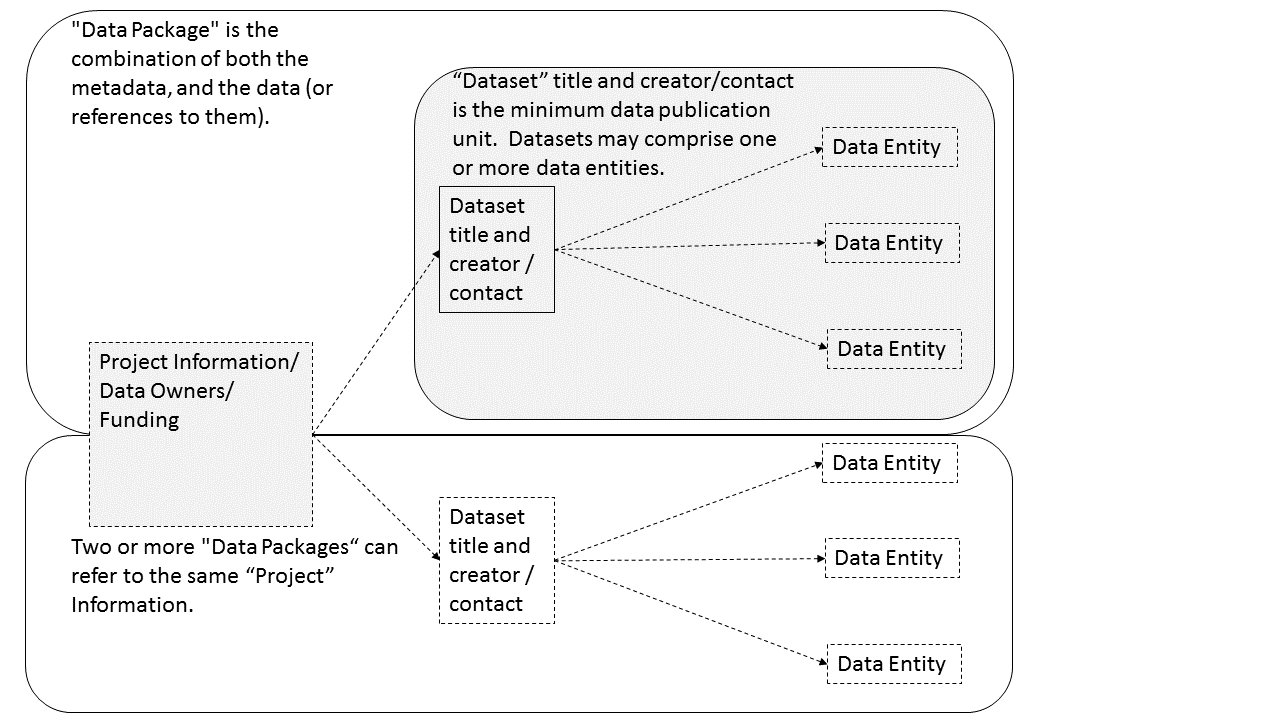
\includegraphics{images/EML_project.png}
\caption{The EML approach to managing Projects, Datasets and Entities}
\label{fig:emlproj}
\end{figure}

\subsection{Procedures when conducting a reproducible research
analysis}\label{procedures-when-conducting-a-reproducible-research-analysis}

Having defined above the principle components for a pipeline there are
procedural questions about how to go about compiling those. The key
steps include:

\begin{itemize}
\itemsep1pt\parskip0pt\parsep0pt
\item  Data Management Plans and Data Inventories
\item  Planning and implementing a pipeline
\item  Tracking method steps
\end{itemize}

These three topics will be explored in each of the next three sections of this report.

\section{Data management plan and data
inventory}\label{data-management-plan-and-data-inventory}

In eco-social epidemiology there is a need for a data management plan
and a data inventory that enables individual scientists, or
multidisciplinary teams of scientists, to manage large and heterogeneous
collections of disparate data sources efficiently. Keeping track of all
the elements of a linked health, social and environmental database is
very challenging, despite major improvements in data management
software, web-portals and virtual laboratories \citep{Fleming2014}.

Effective data management policies and procedures are essential in
managing data-related risk. Such risks include data loss or corruption,
technological obsolescence, breaches of privacy or copyright, and errors
or misuse. 

Data management plans are needed for developing procedures and processes
to keep data safe. There is an issue when ensuring that all relevant
data are collected in deciding what is relevant. Keeping an up-to-date
data inventory and careful organisation of all folders and files helps
mitigate these problems.

Whether data management is the responsibility of the individuals
collecting or collating it, or of the lead scientist, clarity on how and
where data are stored and who manages it is vital, as is a `succession
plan' that sets out the vision of the data collections preservation and
re-use into the future.

\subsection{Data storage and access}\label{data-storage-and-access}

Some datasets such as sensitive personal information about suicide or
climate change scenarios with restrictions due to privacy and
confidentiality rules, or because of protected intellectual property,
need to be accessed in a restricted way. This complicates the
implementation of the method of pipelines which dictates that all the
steps, models and assumptions need to be made transparent and available
for scientific debate even though the datasets may require authorisation
to access. Restrictions around access to data have increased recently in
Australia. As an example the custodians of the national mortality
database made it virtually impossible to access these data for several
years after the discovery of an incident in which Australian population
health researcher Dr Stephen Begg was reported to have hacked into the
database in an illegal act \citep{OKeefe2007}. The subsequent investigation
by the data custodians led to a wide ranging modification to the
procedures for approval and provision of these data that make the access
much more restricted. Appropriate access to data is therefore required
to address this issue. In the work reported in the conference
presentation in this thesis, a range of available workflow tools for
data management and analysis were investigated and developed.

The key components of the  data management system as identified above are shown graphically in figure 
\ref{fig:file_name}.  A project can contain many datasets (folders), which in turn may hold many entities (files). This organisation model for a project can be described in terms of 'general' projects (about general contextual data, accessible to the entire group) or 'specific' projects (about a specific Health/Exposure study and will have a specific subset of authorised people who can access it).  General data can go into the main storage folder however specific data needs to more secure storage.

\begin{figure}[!h]
\centering
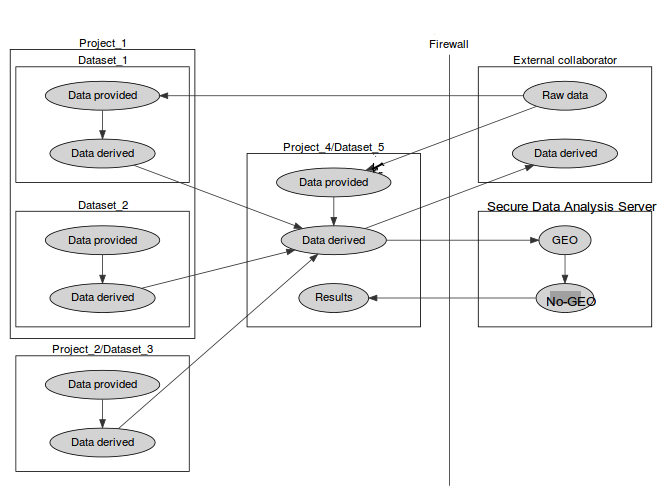
\includegraphics[width=.8\textwidth]{images/file_name.png}
\caption{A schematic diagram of the management of large multi-institute collaborative project}
\label{fig:file_name}
\end{figure}

\subsection{Case study 1: EML and folder structure}

In figure \ref{fig:M2} the conceptual framework described above is implemented in a standardised folder structure.  The main storage location for this data collection is called 'Research data'.  
This computer drive is then structured in a simple hierarchy of projects (folders), datasets (sub-folders) and entities (sub-sub-folders or individual files).  Entities may be individual files, or groups of files in a sub-sub-folder to cater for data structures such as those where there are a collections of files that make up a single entity such as the Shapefile or Raster Image dataset as used in Geographical Information Systems (GIS) software.  As seen in figure \ref{fig:file_name} it might make sense to group all entities into folders that delineate those files provided as raw data and those that were derived by some process within the project.

\begin{figure}[!h]
\centering
\begin{tikzpicture}[dirtree] % it's what we defined above
  
\node [draw=black!50,dashed,rectangle]{{Research data} }
      child { node {{Project} }
          child { node {{Dataset}} 
              child { node {{Entity}} }
          }
          child { node {{Dataset}} 
          }
      }
      child { node {{Project} }       
      };
\end{tikzpicture}
\caption{Conceptual framework for grouping data files (entities) within datasets and projects} \label{fig:M2}
\end{figure}

\newpage

\section{Planning and implementing a
pipeline}\label{planning-and-implementing-a-pipeline}

It can be much easier to conceptualise a complicated data analysis
method than to implement this as a reproducible research pipeline. The
most effective way to implement a pipeline is by methodically tracking
each of the steps taken, the data inputs needed and all the outputs of
the step. If done in a disciplined way then the analyst or some other
person could `audit' the procedure easily and access the details of the
pipeline they need to scrutinise.

\subsection{A standardised data analysis pipeline
framework}\label{a-standardised-data-analysis-pipeline-framework}

One method that was selected for use in the papers of this thesis was
the concept of the Load-Clean-Functions-Do (LCFD) framework. This was
first proposed by Josh Reich on the open-source software discussion
forum called `stack overflow'
(\url{http://stackoverflow.com/a/1434424}), and then encoded into the
`makeProject' R package
(\url{http://cran.r-project.org/web/packages/makeProject/makeProject.pdf}).
The approach is demonstrated in case study 2 below.



\subsection{Case study 2: Simple pipeline using the makeProject
package}\label{case-study-2-simple-pipeline-using-the-makeproject-package}

\begin{Shaded}
\begin{Highlighting}[]
\CommentTok{# in an interactive R session at the command line choose your project directory}
\KeywordTok{setwd}\NormalTok{(}\StringTok{"~/projects"}\NormalTok{)   }
\CommentTok{# load the required functions from the makeProject package}
\KeywordTok{library}\NormalTok{(makeProject)}
\CommentTok{# use the makeProject function to }
\KeywordTok{makeProject}\NormalTok{(}\StringTok{"my_first_pipelines_project"}\NormalTok{)}

\NormalTok{### gives}
\NormalTok{/my_first_pipelines_project/}
\StringTok{    }\ErrorTok{/}\NormalTok{code/}\ErrorTok{**}\NormalTok{.R}
    \NormalTok{/data/}
\StringTok{    }\ErrorTok{/}\NormalTok{DESCRIPTION}
    \NormalTok{/main.R}

\CommentTok{# in main.R you put these lines into the script}
\CommentTok{# and run them as the steps of the pipeline evolve}
\KeywordTok{source}\NormalTok{(}\StringTok{"code/load.R"}\NormalTok{)}
\KeywordTok{source}\NormalTok{(}\StringTok{"code/clean.R"}\NormalTok{)}
\KeywordTok{source}\NormalTok{(}\StringTok{"code/func.R"}\NormalTok{)}
\KeywordTok{source}\NormalTok{(}\StringTok{"code/do.R"}\NormalTok{)}

\CommentTok{# Reporting is then a matter of choice}
\NormalTok{## If using the rmarkdown approach there would be an Rmd file that contained the prose}
\NormalTok{## and turned into a PDF, HTML or Word document with a line such as }
\NormalTok{rmarkdown::}\KeywordTok{render}\NormalTok{(}\StringTok{"My-Pipeline-Report.Rmd"}\NormalTok{, }\StringTok{"pdf_document"}\NormalTok{)}
\end{Highlighting}
\end{Shaded}

\subsection{File organization and
naming}\label{file-organization-and-naming}

In many stages of a pipeline, an analyst will want to include details of
the settings or what dataset they started out with. Rather than saving a
folder or file name that is long and uninformative there are many
different ways to organizing folders and files.

Key techniques for this are available and known in the data analysis
community as `Tidy Data' guidelines. In the words of \citet{WickhamRstudio2014} the
order that data should be arranged in follows some generic principles:

\begin{quote}
'A good ordering makes it easier to scan the raw values. One way of
organizing variables is by their role in the analysis: are values
fixed by the design of the data collection, or are they measured
during the course of the experiment? Fixed variables describe the
experimental design and are known in advance. Computer scientists
often call fixed variables dimensions, and statisticians usually
denote them with subscripts on random variables. Measured variables
are what we actually measure in the study. Fixed variables should come
first, followed by measured variables, each ordered so that related
variables are contiguous. Rows can then be ordered by the first
variable, breaking ties with the second and subsequent (fixed)
variables.'
\end{quote}

\subsubsection{An exemplar}\label{an-exemplar}

The following protocol was developed for an ecology and biodiversity
database that the author of this PhD thesis was involved with. The
naming convention relied heavily on a sequence of information being used
to order the names of folders, subfolders and files. This is:

\begin{enumerate}
\def\labelenumi{\arabic{enumi}.}
\itemsep1pt\parskip0pt\parsep0pt
\item
  The project name (and optional sub-project name)
\item
  Data type (such as experimental unit, observational unit, and/or
  measurement methods)
\item
  Geographic location (State, Country)
\item
  Temporal frequency and coverage (such as annual or seasonal tranches).
\end{enumerate}

\subsubsection{The concepts of slow moving dimensions and fast moving
variables}\label{the-concepts-of-slow-moving-dimensions-and-fast-moving-variables}

The concept of dimensions and variables can be useful here, and
especially for deciding on filenames. Dimensions are fixed or change
slowly while variables change more quickly. By `change', this means that
there are more of them. For example the project name is `fixed', that is
it does not change across the files, but the sub-project name does
change, just more slowly (say there may be 2-3 different sub-projects
within a project). Then there may be a set of data types, and these
`change' more quickly than the sub-project name. Then the geographic and
temporal variables might change quickest of all.

So a general rule for the order of things can be stated. The fixed and
slowly changing variables should come first (those things that don't
change, or don't change much), followed by the more fluid variables (or
things that change more across the project). List elements can then be
ordered so that the groups of things that are similar will always be
contiguous, and vary sequentially within clusters.

An example is shown in Table \ref{tab:TableFiles} to describe this and
make it easier to understand. Here is a set of file names that were
constructed for an ecological field sites project that the I worked on
(\href{http://www.supersites.net.au/}{\url{http://www.supersites.net.au/}}).
That project involved ecological data sampled at plot-based measurement
locations. At the begining of the procedure a controlled vocabulary of
data types and their acronyms was created.

\begin{table}[!h]
\tiny
\centering
\caption{An example of standardised filename conventions to simplify tracking complicated datasets} 
\label{tab:TableFiles}
\begin{tabular}{p{3.3in}p{3in}}
  \hline
Filename & Title \\ 
  \hline
asn\_fnqr\_soil\_charact\_robson\_2011.csv & Soil Data, Far North Queensland Rainforest SuperSite, Robson Creek, 2011 \\ 
  asn\_fnqr\_soil\_pit\_robson\_2012.csv & Soil Pit Data, Water Content and Temperature, Far North Queensland Rainforest SuperSite, Robson Creek, 2012 \\ 
  asn\_fnqr\_veg\_seedling\_robson\_2010-2012.csv & Seedling Survey,  Far North Queensland Rainforest SuperSite, Robson Creek, 2010-2012 \\ 
  asn\_fnqr\_veg\_seedling\_transect\_coord\_robson\_2010-2012.csv & Seedling Survey,  Far North Queensland Rainforest SuperSite, Robson Creek, 2010-2012 \\ 
  asn\_fnqr\_core\_1ha\_robson\_2014.csv & Soil Pit Data, Soil Characterisation, Far North Queensland Rainforest SuperSite, Robson Creek, Core 1 ha plot, 2014 \\ 
  asn\_fnqr\_fauna\_biodiversity\_ctbcc\_2012.csv & Vertebrate Fauna Biodiversity Monitoring, Far North Queensland Rainforest SuperSite, CTBCC, 2012 \\ 
  asn\_fnqr\_fauna\_biodiversity\_ctbcc\_2013.csv & Vertebrate Fauna Biodiversity Monitoring, Far North Queensland Rainforest SuperSite, CTBCC, 2013 \\ 
  asn\_fnqr\_fauna\_biodiversity\_ctbcc\_capetrib\_2014.csv & Avifauna Monitoring, Far North Queensland Rainforest SuperSite, Cape Tribulation, 2014 \\ 
  asn\_fnqr\_fauna\_biodiversity\_ctbcc\_lu11a\_2014.csv & Vertebrate Fauna Biodiversity Monitoring, Far North Queensland Rainforest SuperSite, CTBCC, LU11A, 2014 \\ 
  asn\_fnqr\_fauna\_biodiversity\_ctbcc\_lu7a\_2014.csv & Vertebrate Fauna Biodiversity Monitoring, Far North Queensland Rainforest SuperSite, CTBCC, LU7A, 2014 \\ 
  asn\_fnqr\_fauna\_biodiversity\_ctbcc\_lu7b\_2014.csv & Vertebrate Fauna Biodiversity Monitoring, Far North Queensland Rainforest SuperSite, CTBCC, LU7B, 2014 \\ 
  asn\_fnqr\_fauna\_biodiversity\_ctbcc\_lu9a\_2014.csv & Vertebrate Fauna Biodiversity Monitoring, Far North Queensland Rainforest SuperSite, CTBCC, LU9A, 2014 \\ 
  asn\_fnqr\_fauna\_biodiversity\_ctbcc-lu11a\_2009-2011.csv & Vertebrate Fauna Biodiversity Monitoring, Far North Queensland Rainforest SuperSite, CTBCC, LU11A, 2009-2011 \\ 
  asn\_fnqr\_fauna\_biodiversity\_ctbcc-lu7a\_2009-2011.csv & Vertebrate Fauna Biodiversity Monitoring, Far North Queensland Rainforest SuperSite, CTBCC, LU7A, 2009-2011 \\ 
  asn\_fnqr\_fauna\_biodiversity\_ctbcc-lu9a\_2009-2011.csv & Vertebrate Fauna Biodiversity Monitoring, Far North Queensland Rainforest SuperSite, CTBCC, LU9A, 2009-2011 \\ 
  asn\_fnqr\_fauna\_biodiversity\_habitat\_codes\_ctbcc-lu11a\_2009-2011.pdf & Vertebrate Fauna Biodiversity Monitoring, Far North Queensland Rainforest SuperSite, CTBCC, LU11A, 2009-2011 \\ 
   \hline
\end{tabular}
\end{table}

%\clearpage

\section{Tracking method steps: Visualisation techniques}\label{visualisation-techniques}

\subsection{Make a list of steps, inputs and
outputs}\label{make-a-list-of-steps-inputs-and-outputs}

A very simple example of a pipeline is shown in Table
\ref{tab:TablePipe1}. The steps and data listed in Table
\ref{tab:TablePipe1} can be visualised using the \texttt{newnode}
function described below in case study 3. This creates the graph of this
pipeline shown in Figure \ref{fig:FigSteps}. As the analysis progresses
through the phases of testing, refinement and final versions. The linked
table and graphical depiction can be very helpful for reference by the
analyst. The optional setting to define a status of each step (TODO,
DONE, WONTDO) can be used to add colour, and show steps that remain to
be done. The addition of short summary descriptions are also very useful
for orienting oneself to the required tasks and their priorities. Such
flow chart diagrams can be printed up on large sheets of paper and stuck
on the wall beside a computer workstation for use in day-to-day work.

\begin{table}[!ht]
\centering
\caption{A table with the steps of a simple data analysis pipeline} 
\label{tab:TablePipe1}
\begin{tabular}{p{.6in}p{1.3in}p{1.2in}p{2in}p{1in}}
  \hline
STEP & INPUTS & OUTPUTS & DESCRIPTION & STATUS \\ 
  \hline
Step1 & Source 1, Source 2 & Derived 1, QC check & This might be latitude and longitude of sites & DONE \\ 
  Step2 & Source 3 & Derived 2 & This might be weather data & DONE \\ 
  Step3 & Derived 1, Derived 2 & Derived 3 & Merging these data means they can be analysed & TODO \\ 
  Step4 & Derived 3 & Model selection &  & TODO \\ 
  Step5 & Model selection & Sensitivity analysis &  & TODO \\ 
   \hline
\end{tabular}
\end{table}

\begin{figure}[!h]
\centering
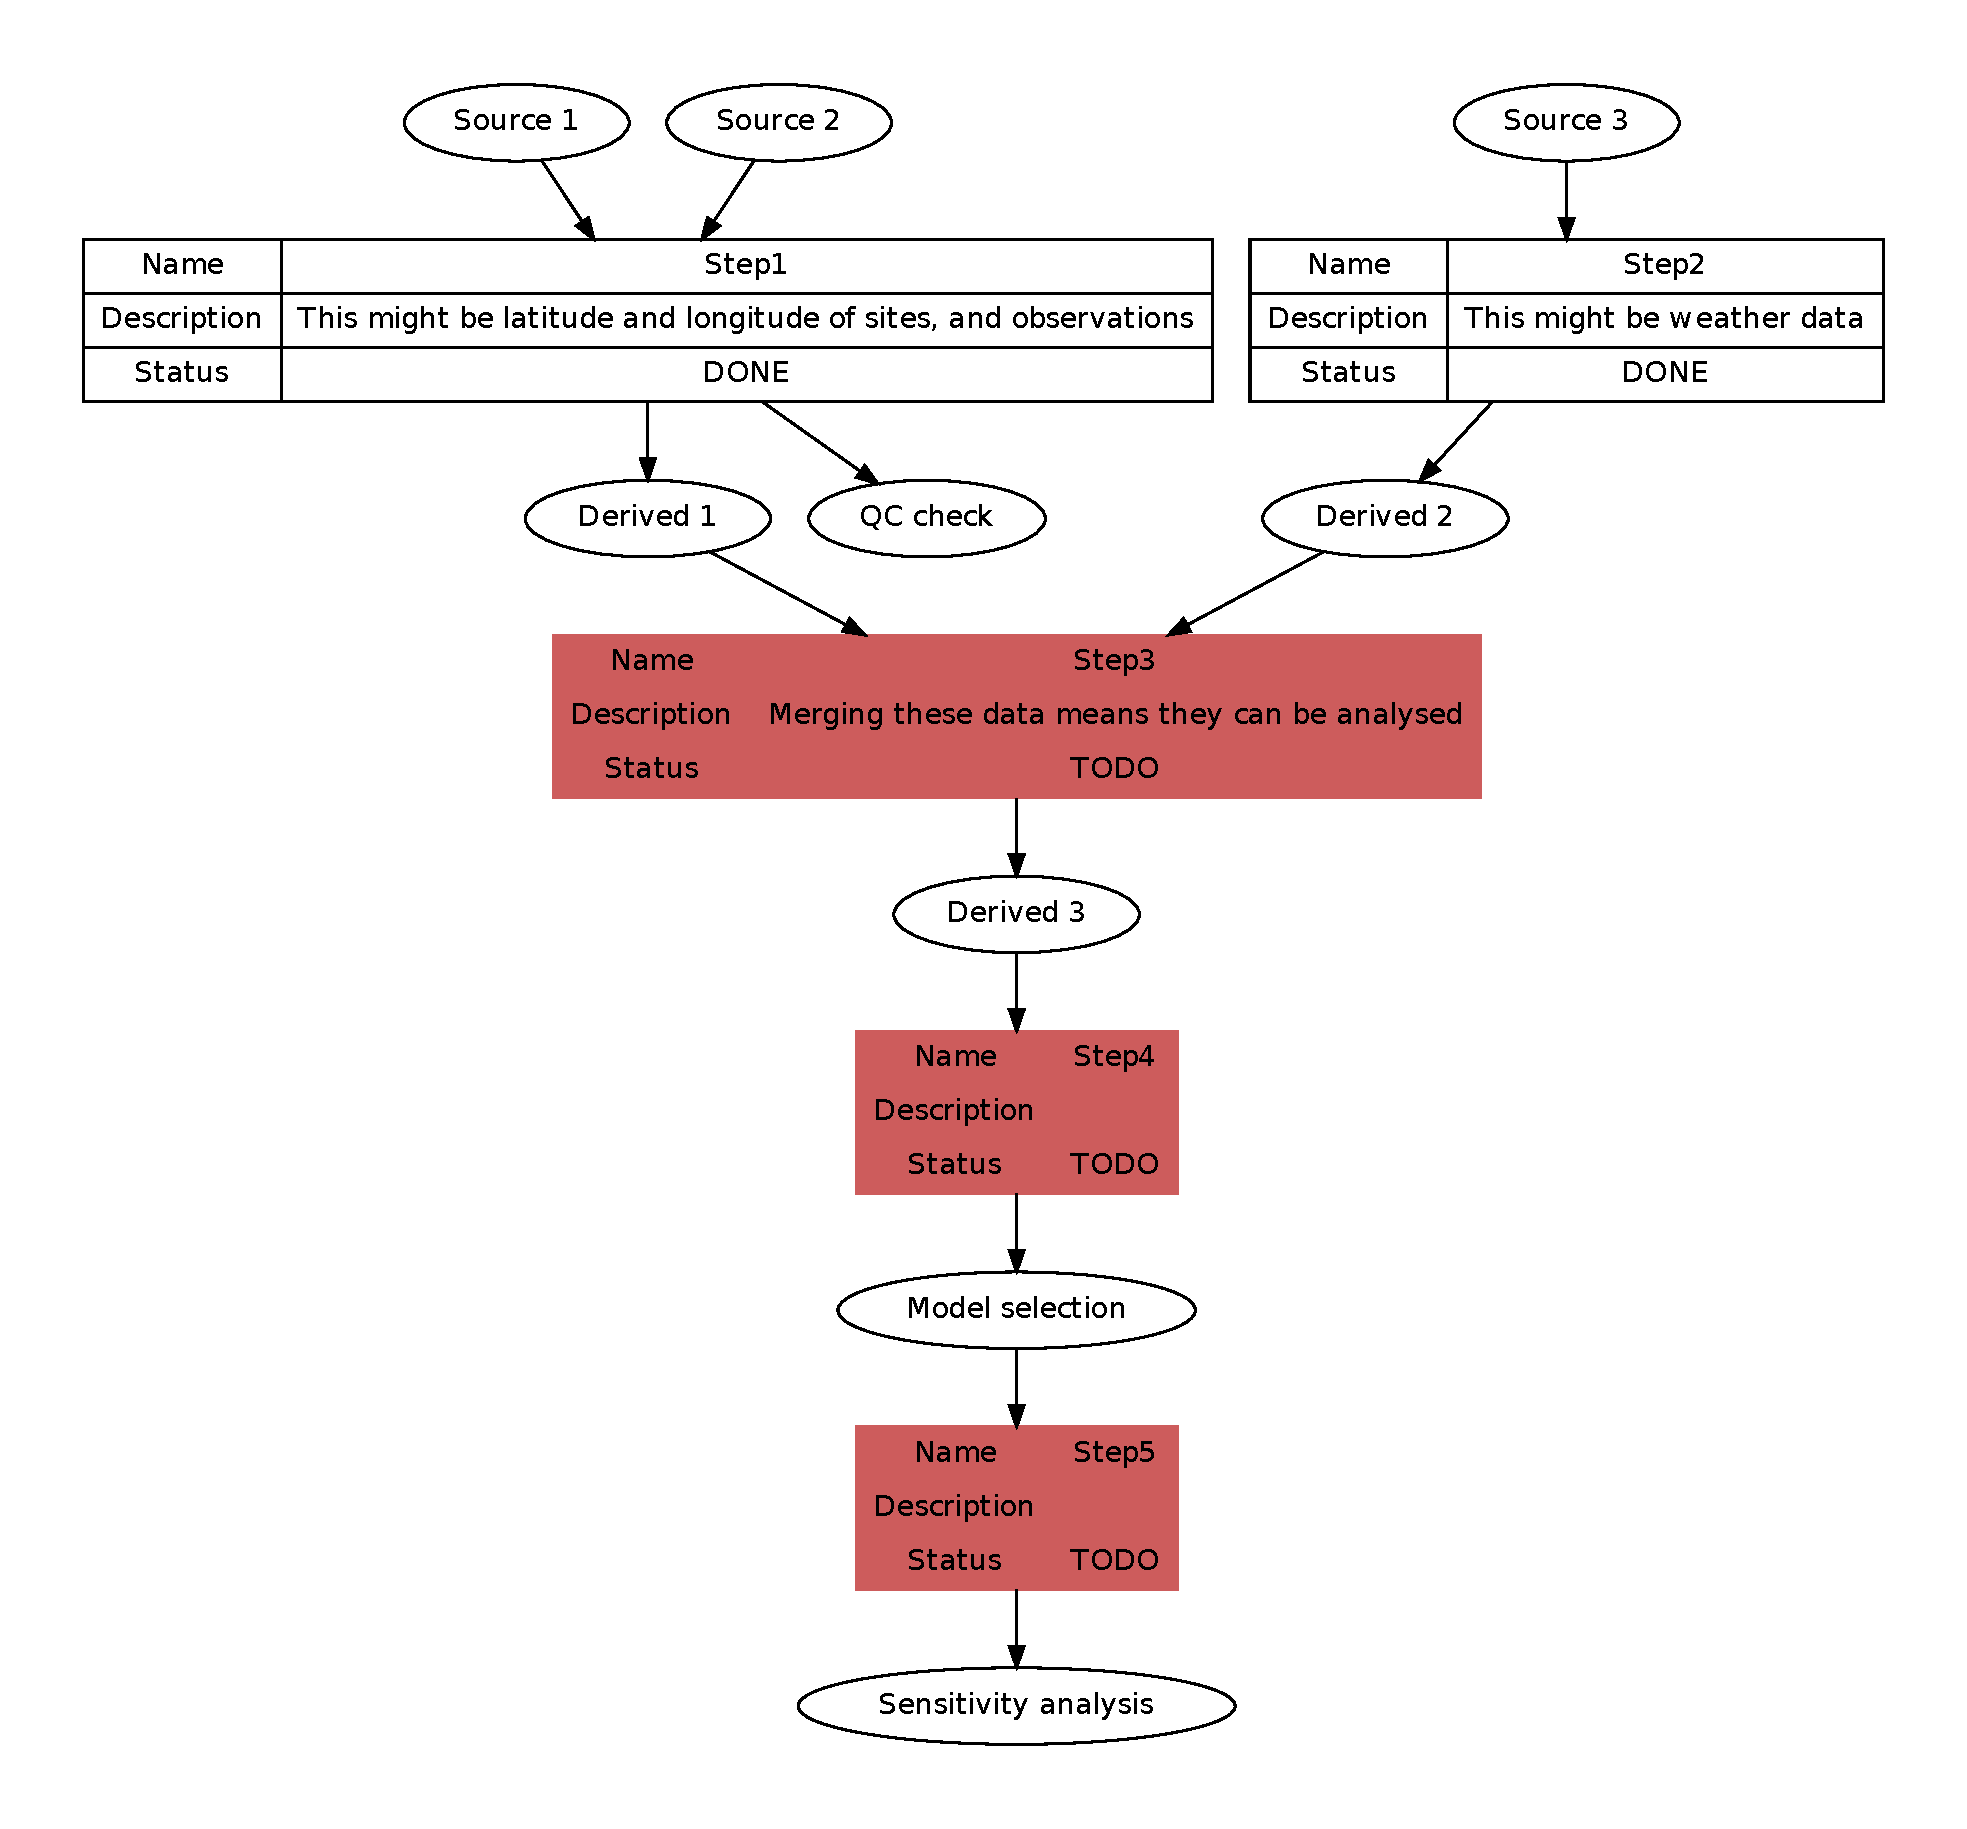
\includegraphics[width=\textwidth]{images/steps-fig1.pdf}
\caption{A visualisation of a data analysis pipeline showing the use of colour}
\label{fig:FigSteps}
\end{figure}

\clearpage

As an example of the kinds of tangible steps such a workflow might
entail a schematic diagram has been created and is shown in Figure
\ref{fig:envepi_data_pipeline.png}.

\begin{figure}[!h]
\centering
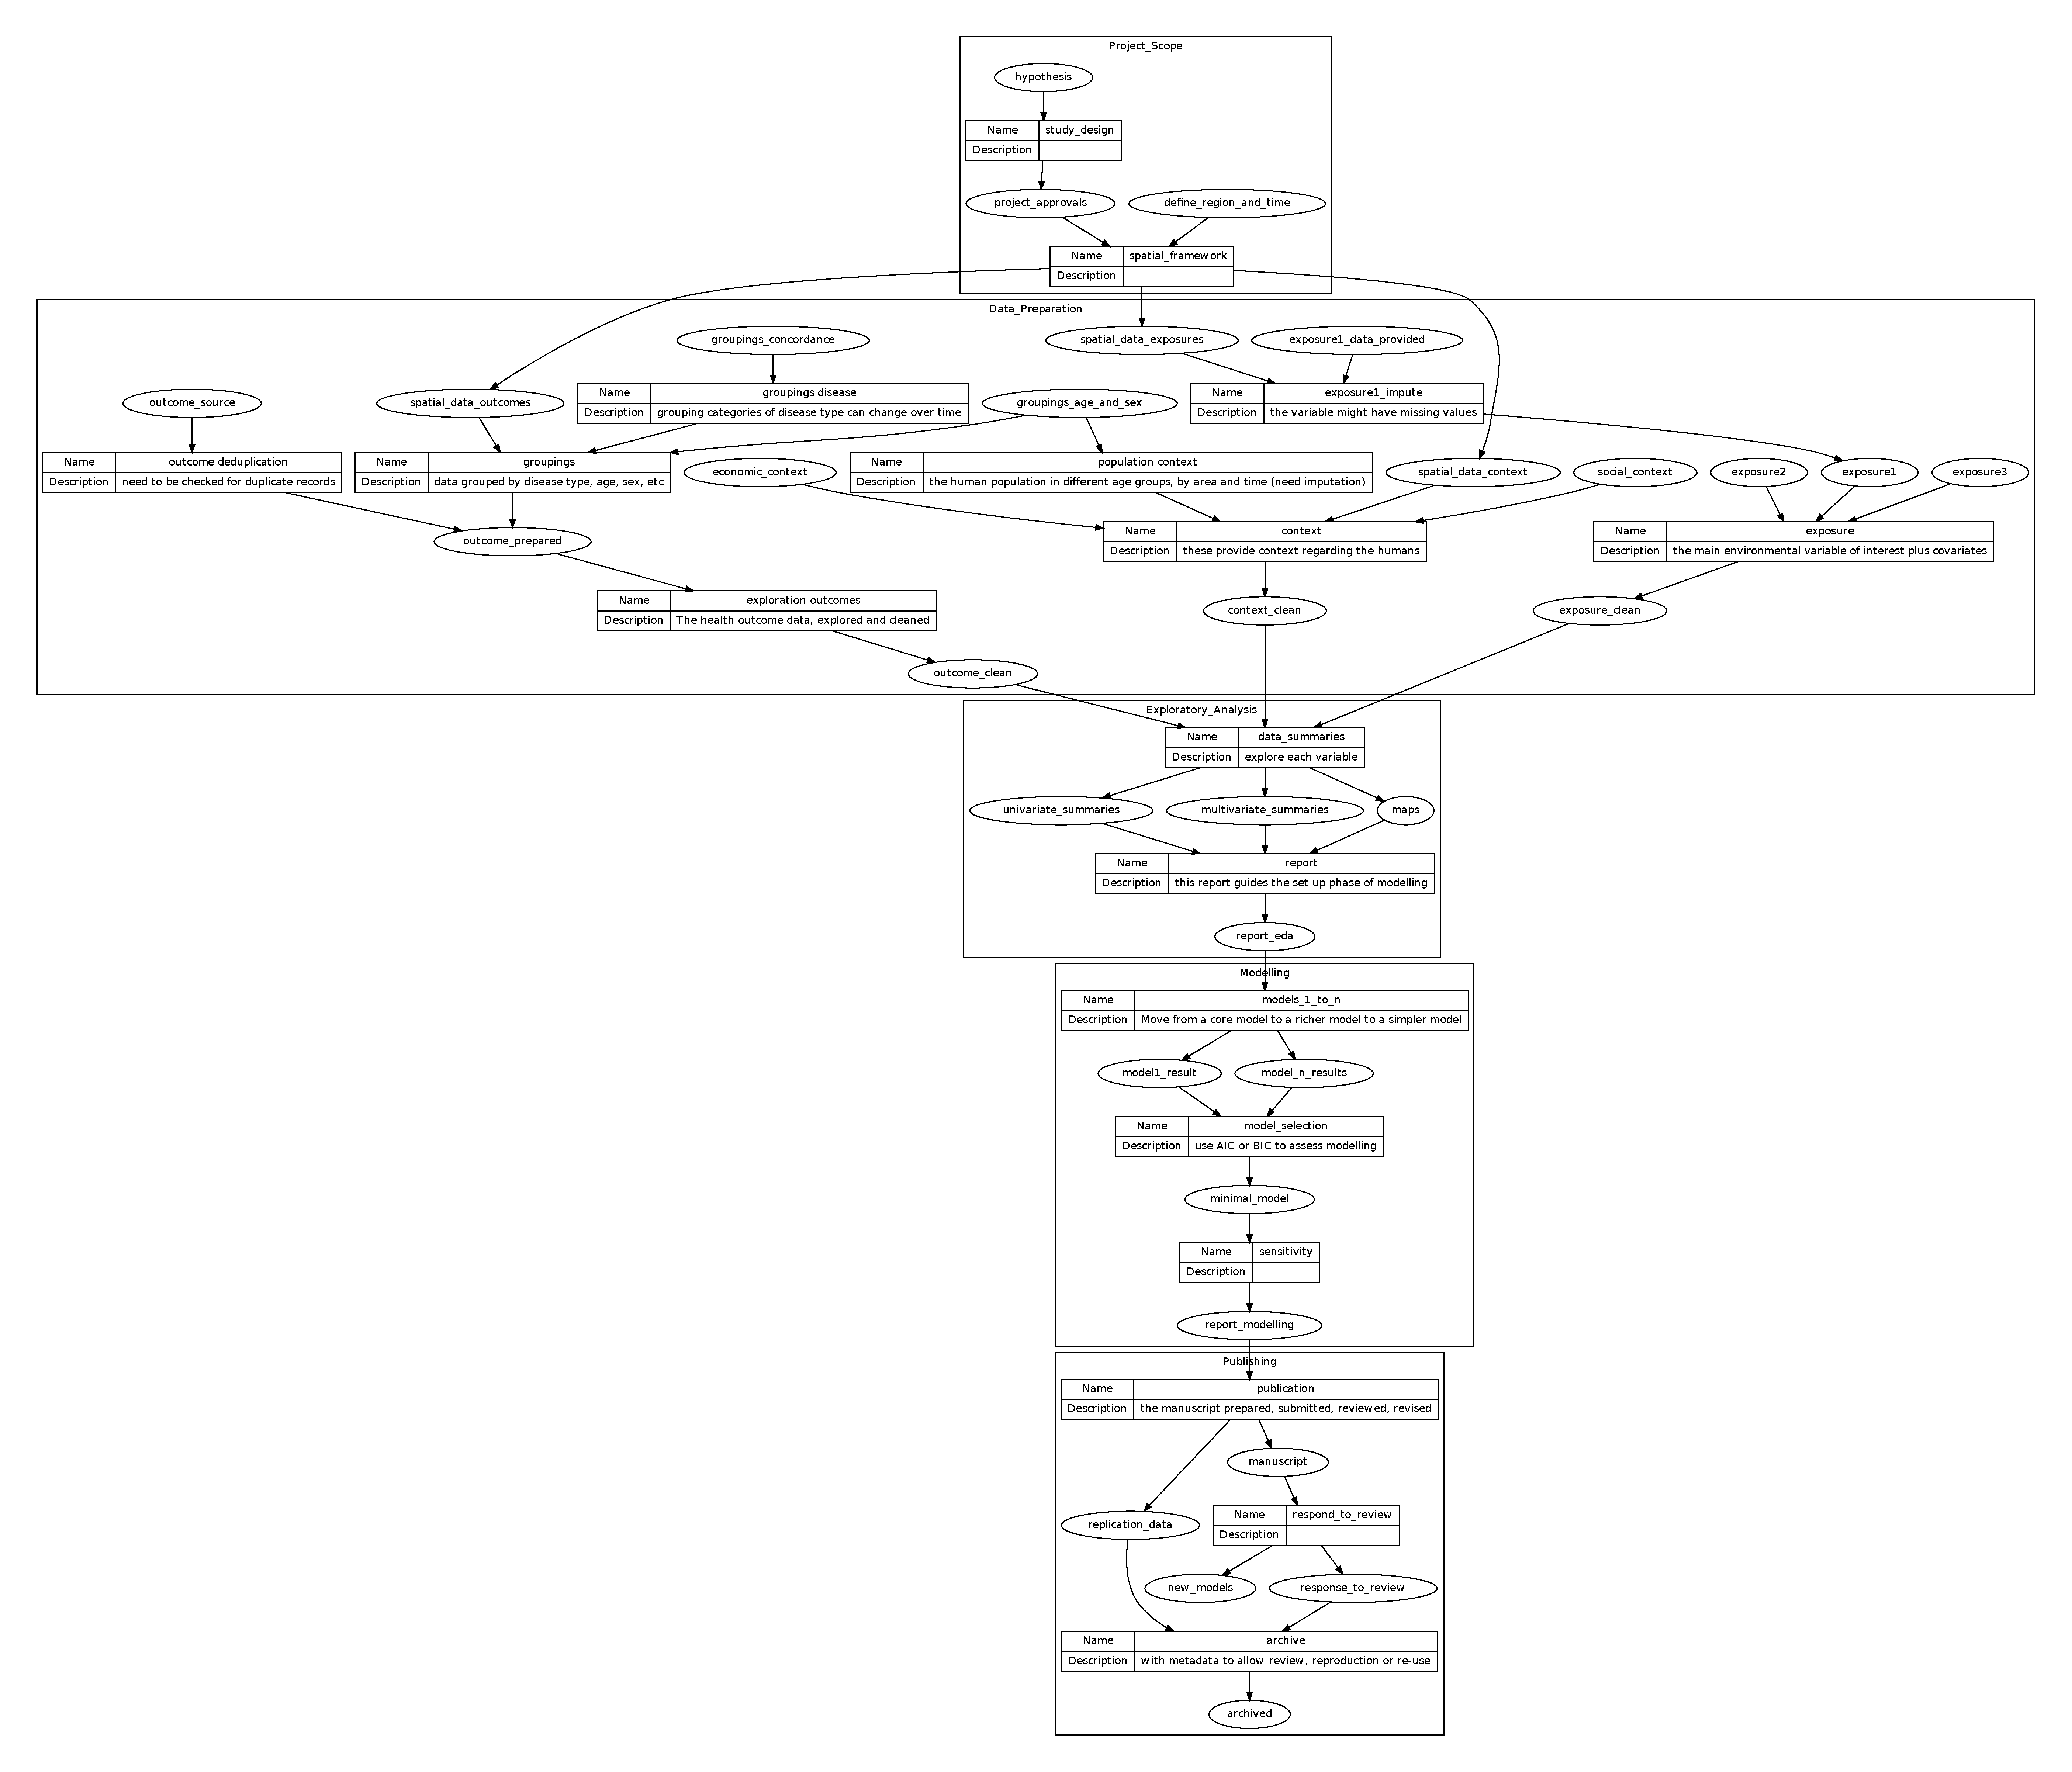
\includegraphics[width=\textwidth]{images/envepi_data_pipeline.pdf}
\caption{A schematic flow chart showing the steps required to prepare and
conduct an analysis of health, environmental and social data.}       
\label{fig:envepi_data_pipeline.png}
\end{figure}

A high resolution version of this image is available online at
\href{https://github.com/swish-climate-impact-assessment/swish_data_management_procedures/blob/phd_appendix/images/envepi_data_pipeline.pdf}{\url{https://github.com/swish-climate-impact-assessment/swish_data_management_procedures/blob/phd_appendix/images/envepi_data_pipeline.pdf}}

\subsection{Case study 3: Visualisation of methods steps using bespoke
software}\label{case-study-3-visualisation-of-methods-steps-using-bespoke-software}

The method step is the key atomic unit of a scientific pipeline. It
consists of inputs, outputs and a rationale for why the step is taken.

A simple way to keep track of the steps, inputs and outputs is shown in
Table \ref{tab:TableBasic}.

\begin{table}[!h]
\centering
\caption{A simple table to track method steps, data inputs and outputs} 
\label{tab:TableBasic}
\begin{tabular}{p{.6in}p{2in}p{2in}}
  \hline
STEP & INPUTS & OUTPUTS \\ 
  \hline
Step1 & Input 1, Input 2 & Output 1 \\ 
  Step2 & Input 3 & Output 2 \\ 
  Step3 & Output 1, Output 2 & Output 3 \\ 
   \hline
\end{tabular}
\end{table}

The steps and data listed in Table \ref{tab:TableBasic} can be
visualised. To achieve this an R function was written as part of this
PhD project and is distributed in the author's own R package available
on Github (\url{https://github.com/ivanhanigan/disentangle}). This is
the \texttt{newnode} function. The function returns a string of text
written in the \texttt{dot} language which can be rendered in R using
the \texttt{DiagrammeR} package, or the standalone \texttt{graphviz}
package. This creates the graph view shown in Figure \ref{fig:FigBasic}.
Note that a new field was added for Descriptions as these are highly
recommended.

\begin{Shaded}
\begin{Highlighting}[]
\KeywordTok{library}\NormalTok{(disentangle); }\KeywordTok{library}\NormalTok{(stringr); }\KeywordTok{library}\NormalTok{(readxl)}
\NormalTok{steps <-}\StringTok{ }\KeywordTok{read_excel}\NormalTok{(}\StringTok{"steps_basic_workflow.xlsx"}\NormalTok{)}
\NormalTok{nodes <-}\StringTok{ }\KeywordTok{newnode}\NormalTok{(}\DataTypeTok{indat =} \NormalTok{steps, }\DataTypeTok{names_col =} \StringTok{"STEP"}\NormalTok{,}
                 \DataTypeTok{in_col =} \StringTok{"INPUTS"}\NormalTok{,}\DataTypeTok{out_col =} \StringTok{"OUTPUTS"}\NormalTok{)}
\NormalTok{DiagrammeR::}\KeywordTok{grViz}\NormalTok{(nodes)}
\end{Highlighting}
\end{Shaded}

\begin{figure}[!ht]
\centering
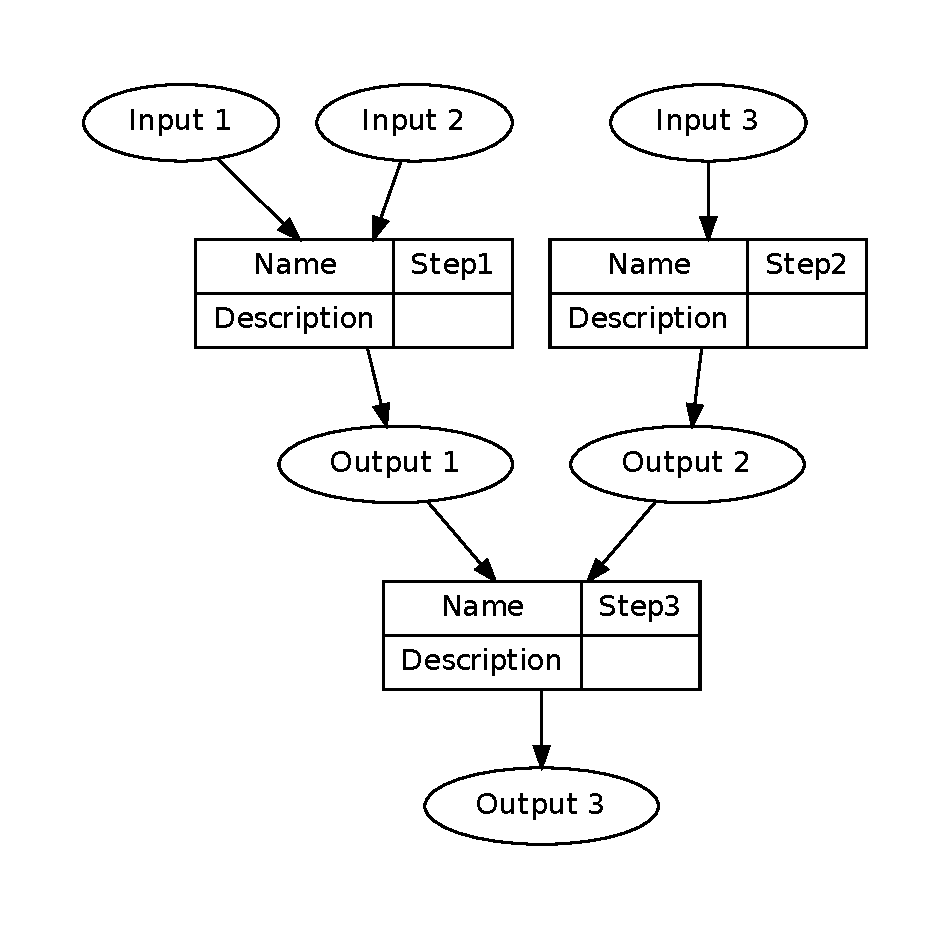
\includegraphics[width=.5\textwidth]{images/fig-basic.pdf}
\caption{A graphical view of the steps that comprise a simple data analysis pipeline}
\label{fig:FigBasic}
\end{figure}

\clearpage
\renewcommand\refname{{References for appendix 2}} 
%\bibliographystyle{plainnat}
%\bibliography{/home/ivan_hanigan/references/library}

\begin{thebibliography}{30}
\providecommand{\natexlab}[1]{#1}
\providecommand{\url}[1]{\texttt{#1}}
\expandafter\ifx\csname urlstyle\endcsname\relax
  \providecommand{\doi}[1]{doi: #1}\else
  \providecommand{\doi}{doi: \begingroup \urlstyle{rm}\Url}\fi

\bibitem[Barnett and Dobson(2010)]{Barnett2010}
Adrian~G. Barnett and Annette~J. Dobson.
\newblock \emph{{Analysing Seasonal Health Data}}.
\newblock Springer, Berlin, Heidelberg, Germany, 2010.

\bibitem[Barnett et~al.(2014)Barnett, Baker, and Dobson]{Barnett2015}
Adrian~G. Barnett, Peter Baker, and Annette~J Dobson.
\newblock {Package ‘season': Analysing seasonal data R functions. R package
  version 0.3-5}, 2014.

\bibitem[Bodnar et~al.(2004)Bodnar, Castorina, Desai, Duramad, Fischer,
  Klepeis, Liang, Mehta, Naumoff, Noth, Schei, Tian, Vork, and
  Smith]{Bodnar2004}
Agnes Bodnar, Rosemary Castorina, Manish Desai, Paurene Duramad, Susan Fischer,
  Neil Klepeis, Song Liang, Sumi Mehta, Kyra Naumoff, Elizabeth~M Noth, Morten
  Schei, Linwei Tian, Kathleen~L Vork, and Kirk~R Smith.
\newblock {Lessons learned from "the skeptical environmentalist": an
  environmental health perspective.}
\newblock \emph{International journal of hygiene and environmental health},
  207\penalty0 (1):\penalty0 57--67, 2004.
\newblock \doi{10.1078/1438-4639-00265}.

\bibitem[Borer et~al.(2009)Borer, Seabloom, Jones, and Schildhauer]{Borer2009a}
Elizabeth~T. Borer, Eric~W. Seabloom, Matthew~B. Jones, and Mark Schildhauer.
\newblock {Some simple guidelines for effective data management}.
\newblock \emph{Bulletin of the Ecological Society of America}, \penalty0
  \penalty0 205--214, 2009.
\newblock URL
  \url{http://www.esajournals.org/doi/abs/10.1890/0012-9623-90.2.205}.

\bibitem[Cai et~al.(2010)Cai, Cowan, Braganza, Jones, and Risbey]{Cai2010}
Wenju Cai, Tim Cowan, Karl Braganza, David Jones, and James Risbey.
\newblock {Comment on 'On the recent warming in the Murray Darling Basin: Land
  surface interactions misunderstood' by Lockart et al.}
\newblock \emph{Geophysical Research Letters}, 37\penalty0 (10):\penalty0 1--3,
  may 2010.
\newblock \doi{10.1029/2009GL042254}.

\bibitem[Fleming et~al.(2014)Fleming, Haines, Golding, Kessel, Cichowska,
  Sabel, Depledge, Sarran, Osborne, Whitmore, Cocksedge, and
  Bloomfield]{Fleming2014}
Lora Fleming, Andy Haines, Brian Golding, Anthony Kessel, Anna Cichowska, Clive
  Sabel, Michael Depledge, Christophe Sarran, Nicholas Osborne, Ceri Whitmore,
  Nicola Cocksedge, and Daniel Bloomfield.
\newblock {Data mashups: Potential contribution to decision support on climate
  change and health}.
\newblock \emph{International Journal of Environmental Research and Public
  Health}, 11\penalty0 (2):\penalty0 1725--1746, 2014.
\newblock \doi{10.3390/ijerph110201725}.

\bibitem[Gentleman and {Temple Lang}(2004)]{Gentleman2004}
Robert Gentleman and Duncan {Temple Lang}.
\newblock {Statistical Analyses and Reproducible Research}.
\newblock \emph{Journal of Computational and Graphical Statistics}, 16\penalty0
  (1):\penalty0 1--23, mar 2004.
\newblock \doi{10.1198/106186007X178663}.

\bibitem[Healy(2013)]{Healy2013}
Kieran Healy.
\newblock {Choosing Your Workflow Applications}, 2013.
\newblock URL \url{https://github.com/kjhealy/workflow-paper}.

\bibitem[Leek and Peng(2015{\natexlab{a}})]{Leek2015a}
Jeffrey~T. Leek and Roger~D. Peng.
\newblock {Opinion: Reproducible research can still be wrong: Adopting a
  prevention approach.}
\newblock \emph{Proceedings of the National Academy of Sciences of the United
  States of America}, 112\penalty0 (6):\penalty0 1645--1646,
  2015{\natexlab{a}}.
\newblock \doi{10.1073/pnas.1421412111}.

\bibitem[Leek and Peng(2015{\natexlab{b}})]{Leek2015b}
Jeffrey~T. Leek and Roger~D. Peng.
\newblock {Statistics: P values are just the tip of the iceberg}.
\newblock \emph{Nature}, 520\penalty0 (7549):\penalty0 612--612,
  2015{\natexlab{b}}.
\newblock \doi{10.1038/520612a}.

\bibitem[Long(2008)]{Long2008}
J~Scott. Long.
\newblock \emph{{The workflow of data analysis using Stata}}.
\newblock Stata publishing, 2008.
\newblock ISBN 9781597180474.

\bibitem[McCullough and Heiser(2008)]{McCullough2008}
B.~D. McCullough and David~A. Heiser.
\newblock {On the accuracy of statistical procedures in Microsoft Excel 2007}.
\newblock \emph{Computational Statistics and Data Analysis}, 52\penalty0
  (10):\penalty0 4570--4578, 2008.
\newblock \doi{10.1016/j.csda.2008.03.004}.

\bibitem[McMichael(2013)]{McMichael2013}
Anthony~J. McMichael.
\newblock {Impediments to comprehensive research on climate change and health}.
\newblock \emph{International Journal of Environmental Research and Public
  Health}, 10\penalty0 (11):\penalty0 6096--6105, 2013.
\newblock \doi{10.3390/ijerph10116096}.

\bibitem[Michener et~al.(1997)Michener, Brunt, Helly, Kirchner, and
  Stafford]{Michener1997}
William~K. Michener, James~W. Brunt, John~J. Helly, Thomas~B. Kirchner, and
  Susan~G. Stafford.
\newblock {Nongeospatial metadata for the ecological sciences}.
\newblock \emph{Ecological Applications}, 7\penalty0 (1):\penalty0 330--342,
  1997.

\bibitem[Noble(2009)]{Noble2009}
William~Stafford Noble.
\newblock {A quick guide to organizing computational biology projects}.
\newblock \emph{PLoS Computational Biology}, 5\penalty0 (7):\penalty0 1--5,
  2009.
\newblock \doi{10.1371/journal.pcbi.1000424}.

\bibitem[O'Keefe(2007)]{OKeefe2007}
B~O'Keefe.
\newblock {Hackers pick up UQ cash prize}, 2007.
\newblock URL
  \url{http://www.theaustralian.com.au/higher-education/hackers-pick-up-uq-cas%
h-prize/story-e6frgcjx-1111113191659}.

\bibitem[Peng(2011)]{Peng2011}
Roger~D Peng.
\newblock {Reproducible research in computational science.}
\newblock \emph{Science}, 334\penalty0 (6060):\penalty0 1226--1227, 2011.
\newblock \doi{10.1126/science.1213847}.

\bibitem[Peng(2015)]{Peng}
Roger~D. Peng.
\newblock \emph{{Report writing for data science in R}}.
\newblock Leanpub. Unpublished Draft (Accessed 22 Dec. 2015), 2015.
\newblock URL \url{https://leanpub.com/reportwriting}.

\bibitem[Peng and Dominici(2008)]{Peng2008a}
Roger~D Peng and F~Dominici.
\newblock \emph{{Statistical methods for environmental epidemiology with R. A
  case study in air pollution and health}}.
\newblock Springer Science {\&} Business Media, New York, USA, 2008.

\bibitem[Peng et~al.(2006)Peng, Dominici, and Zeger]{Peng2006}
Roger~D. Peng, Francesca Dominici, and Scott~L. Zeger.
\newblock {Reproducible epidemiologic research}.
\newblock \emph{American Journal of Epidemiology}, 163\penalty0 (9):\penalty0
  783--789, 2006.
\newblock \doi{10.1093/aje/kwj093}.

\bibitem[Pullin and Salafsky(2010)]{Pullin2010}
Andrew~S. Pullin and Nick Salafsky.
\newblock {Save the whales? Save the rainforest? Save the data!}
\newblock \emph{Conservation Biology}, 24\penalty0 (4):\penalty0 915--917,
  2010.
\newblock \doi{10.1111/j.1523-1739.2010.01537.x}.

\bibitem[Schulte et~al.(2012)Schulte, Davison, Dye, and Dominik]{Schulte}
E~Schulte, D~Davison, T~Dye, and C~Dominik.
\newblock {A multi-language computing environment for literate programming and
  reproducible research}.
\newblock \emph{Journal of Statistical Software}, 46\penalty0 (3), 2012.
\newblock URL \url{http://www.jstatsoft.org/v46/i03/paper}.

\bibitem[Schwab et~al.(2000)Schwab, Karrenbach, and Claerbout]{Schwab2000}
M~Schwab, M~Karrenbach, and J~Claerbout.
\newblock {Making scientific computations reproducible}.
\newblock \emph{Computing in Science and Engineering}, 2\penalty0 (6):\penalty0
  61--67, 2000.
\newblock \doi{10.1109/5992.881708}.

\bibitem[Scott(2010)]{Scott}
Theresa~A Scott.
\newblock {Reproducible Research with R, TEX and Sweave}, 2010.
\newblock URL
  \url{http://biostat.mc.vanderbilt.edu/wiki/pub/Main/TheresaScott/Reproducibl%
eResearch.TAScott.handout.pdf}.

\bibitem[Silberzahn and Uhlmann(2015)]{Silberzahn2015}
Raphael Silberzahn and Eric~L. Uhlmann.
\newblock {Crowdsourced research: Many hands make tight work}.
\newblock \emph{Nature}, 526\penalty0 (7572):\penalty0 189--191, 2015.
\newblock \doi{10.1038/526189a}.

\bibitem[S{\'{o}}lymos and Feh{\'{e}}r(2008)]{Solymos2008}
P~S{\'{o}}lymos and Z~Feh{\'{e}}r.
\newblock {The mefa package: a tool for reproducible data processing in
  biogeography}, 2008.
\newblock URL
  \url{http://biogeography.blogspot.com.au/2008/04/mefa-package-tool-for-repro%
ducible-data.html}.

\bibitem[Vines et~al.(2014)Vines, Albert, Andrew, D{\'{e}}barre, Bock,
  Franklin, Gilbert, Moore, Renaut, and Rennison]{Vines2014a}
Timothy~H. Vines, Arianne Y~K Albert, Rose~L. Andrew, Florence D{\'{e}}barre,
  Dan~G. Bock, Michelle~T. Franklin, Kimberly~J. Gilbert, Jean-S{\'{e}}bastien
  Moore, S{\'{e}}bastien Renaut, and Diana~J. Rennison.
\newblock {The availability of research data declines rapidly with article
  age}.
\newblock \emph{Current Biology}, 24\penalty0 (1):\penalty0 94--97, 2014.
\newblock \doi{10.1016/j.cub.2013.11.014}.

\bibitem[White et~al.(2013)White, Baldridge, Brym, Locey, Mcglinn, and
  Supp]{White2013}
Ethan~P White, Elita Baldridge, Zachary~T Brym, Kenneth~J Locey, Daniel~J
  Mcglinn, and Sarah~R Supp.
\newblock {Nine simple ways to make it easier to (re)use your data}.
\newblock 2013.
\newblock \doi{10.7287/peerj.preprints.7v2}.

\bibitem[Wickham(2014)]{WickhamRstudio2014}
Hadley Wickham.
\newblock {Tidy data}.
\newblock \emph{Journal of Statistical Software}, 59\penalty0 (10):\penalty0
  1--23, 2014.
\newblock \doi{10.18637/jss.v059.i10}.

\bibitem[Xie(2014)]{Xie2014a}
Yihui Xie.
\newblock {Chapter 1. Knitr: A comprehensive tool for reproducible research in
  R}.
\newblock In V~Stodden, F~Leisch, and RD~Peng, editors, \emph{Implementing
  Reproducible Research}. CRC Press, Boca Raton, USA, 2014.
\newblock ISBN 978-0-387-98140-6.


\end{thebibliography}


\end{document}
